\documentclass{article}
\usepackage[italian]{babel}
\usepackage[tmargin=2cm,rmargin=1.5in,lmargin=1.5in,margin=0.85in,bmargin=2cm,footskip=.2in]{geometry}
\usepackage{siunitx}
\sisetup{separate-uncertainty=true, per-mode=fraction, parse-numbers=true}
\usepackage{caption}
\usepackage[T1]{fontenc}
\usepackage{bookmark}
\usepackage{mathcomp}
\usepackage{graphicx}
\usepackage{multicol}
\usepackage{booktabs}
\usepackage{amsmath,amsfonts,amsthm,amssymb,mathtools}
\hypersetup{
	pdftitle={Relazione pendolo fisico},
	colorlinks=true, linkcolor=doc!90,
	bookmarksnumbered=true,
	bookmarksopen=true
}
\usepackage{blindtext}
\usepackage{wrapfig}
\usepackage{listings}
\usepackage{xcolor}
\usepackage{float}
\usepackage{amsmath}
\usepackage{amssymb}
\usepackage{tikz}
\usepackage{titling}
\renewcommand\maketitlehooka{\null\mbox{}\vfill}
\renewcommand\maketitlehookd{\vfill\null}
\usepackage{multirow}
\usepackage{biblatex}
\definecolor{codegreen}{rgb}{0,0.6,0}
\definecolor{codegray}{rgb}{0.5,0.5,0.5}
\definecolor{codepurple}{rgb}{0.58,0,0.82}
\definecolor{backcolour}{rgb}{0.95,0.95,0.92}
\definecolor{doc}{rgb}{0,0,0}
\lstdefinestyle{code}{
    backgroundcolor=\color{backcolour},   
    commentstyle=\color{codegreen},
    keywordstyle=\color{magenta},
    numberstyle=\tiny\color{codegray},
    stringstyle=\color{codepurple},
    basicstyle=\ttfamily\footnotesize,
    breakatwhitespace=false,         
    breaklines=true,                 
    captionpos=b,                    
    keepspaces=true,                                     
    showspaces=false,                
    showstringspaces=false,
    showtabs=false,                  
    tabsize=2,
    inputencoding=ansinew,
    extendedchars=true,
    numbers=left,                    
    numbersep=5pt
}

\lstset{style=code}
\usepackage[varbb]{newpxmath}
\usepackage{circuitikz}
\captionsetup{labelfont={bf, sc}}
\title{Relazione pendolo fisico}
\author{Francesco Sermi}
\date{\today}
\begin{document}
	\maketitle
	\section{Scopo}
	Misurare il periodo di oscillazione di un pendolo fisico in funzione della distanza $d$ del punto $P$ in cui esso è vincolato e il centro di massa 
	\section{Premesse teoriche}
	Un corpo rigido fissato ad un punto di sospensione $P$ (che dista $d$ dal centro di massa) e soggetto alla gravità costituisce un pendolo fisico. Se viene spostato di un angolo $\theta$ dalla sua posizione di equilibrio, la gravità effettua un momento torcente sul centro di massa di questo corpo pari a
	$$
		\tau = -mgd\sin{\theta}
	$$
	e utilizzando la seconda equazione cardinale sappiamo che
	\begin{equation*}
		\tau = \frac{dL}{dt}
	\end{equation*}
	e sapendo che in questo caso il momento angolare a pari a $L = I\omega = I \frac{d\theta}{dt}$, abbiamo che
	\begin{equation*}
		\tau = \frac{dL}{dt} = I\ddot{\theta} = -mgd\sin{\theta}
	\end{equation*}
	dove $I$ rappresenta il momento di inerzia rispetto al punto P che, per il teorema di Hyugens-Steiner, risulta essere pari a:
	$$
		I = I_{CM} + md^2 = \frac{ml^2}{12} + md^2
	$$
	dove $m$ è la massa dell'asta, $l$ è la lunghezza complessiva dell'asta e $d$ è la distanza del punto $P$ dal centro di massa. \\
	Per angoli $\theta$ \emph{piccoli} (spiegherò alla fine di questa sezione che cosa si intende), possiamo utilizzare l'ipotesi delle piccole oscillazioni, per cui risulta che
	\begin{equation}
		\left( \frac{ml^2}{12} + md^2 \right) \ddot{\theta} = -mgd\theta \implies \ddot{\theta} = -\frac{gd}{\frac{l^2}{12} + d^2} \theta
	\end{equation}
	Come possiamo notare, quest'equazione differenziale è quella caratterizzante un moto armonico di pulsazione $\omega_0 = \sqrt{\frac{gd}{\frac{l^2}{12} + d^2}}$ dunque il periodo sarà di questo moto sarà banalmente
	\begin{equation}
		T = 2\pi * \sqrt{\frac{ \frac{l^2}{12} + d^2 }{gd}}
	\end{equation}
	Quindi si osserva che il periodo dipende dalla lunghezza dell'asta $l$ e dalla distanza $d$ del centro di massa dal punto di sospensione $P$, che sono due grandezze che ci dobbiamo accingere a misurare. \\
	Prima di procedere, specifichiamo che cosa voglia dire angoli \emph{piccoli}: il periodo, se non utilizziamo l'ipotesi delle piccole oscillazioni attorno al punto di equilibrio, si può dimostrare che essere ricondotto ad un integrale ellittico incompleto di prima specie di cui sappiamo calcolare l'espansione in serie di Taylor, che risulta essere pari a
	\begin{equation}
		T = 2 \pi \sqrt{\frac{\frac{l^2}{12} + d^2}{gd}} \left( 1 + \frac{\theta_0^2}{16} + o(\theta_0^2) \right)
	\end{equation}
	ora se risulta che $\frac{\theta_0^2}{16} \ll \frac{\sigma_T}{T_0}$ allora possiamo trascurare i termini successivi all'ordine zero dello sviluppo in serie, dunque risulta che l'errore dipende esclusivamente dalla lunghezza $l$ dell'asta e dalla distanza $d$ del punto di sospensione dal centro di massa. 
\section{Strumenti e materiali}
	\textbf{Strumenti}:	
	\begin{itemize}
		\item Metro a nastro, con risoluzione pari a $0.1 \, \si{\centi\meter}$
		\item Cronometro con risoluzione pari a $0.01 \, \si{\second}$
	\end{itemize}
	\textbf{Materiali}:
	\begin{itemize}
		\item Asta metallica forata
		\item PC
		\item Supporto per la sospensione
	\end{itemize}
\section{Descrizione delle misure}
Prima di procedere a misurare il periodo delle oscillazioni, ho misurato la lunghezza dell'asta $l$, che risulta essere pari a $l = (104.5 \pm 0.1) \, \si{\centi\meter}$. \\
Per stimare il centro di massa, siccome non posso supporre l'asta omogenea e questa presenta dei fori (quindi il centro di massa non si trova a metà del corpo), ho provato a mettere in equilibrio l'asta facendola sporgere dal banco di lavoro e vedere fin dove l'asta non cadeva. \\
Successivamente ho iniziato a misurare i periodi di oscillazioni in funzione della distanza $d$ del punto di sospensione dal centro di massa del corpo. Per ogni foro, che utilizzavo per tenere sospeso il pendolo, ho misurato $10$ periodi di oscillazione: infatti la maggiore fonte di errori in queste misurazioni deriva dal tempo di reazione con cui io vado a fermare il cronometro. \\
\section{Analisi delle misure}
Come ho accennato nell'analisi delle misure, la misura sul tempo era dominata da errori accidentali dovuti al mio tempo di reazione nel fermare il cronometro. Dunque, ho considerato, come miglior stima del nostro misurando per ogni foro, la media aritmetica dei $10$ periodi di oscillazione che ho misurato e come incertezza ho utilizzato la deviazione standard della media. \\

\begin{wraptable}{r}{0.3\textwidth}
	\centering
	\begin{tabular}{c c} \toprule
		$T_i$ & $\sigma_i$ \\
		$[\si{\second}]$ & $[\si{\second}]$ \\ \toprule
		
	\end{tabular}
\end{wraptable}

\noindent Dunque il periodo di oscillazione del pendolo all'$i$-esimo foro risulta essere pari a
\begin{equation}
	T_i = \left( m_i \pm \sqrt{\frac{1}{10 \cdot 9}\sum_{j=1}^{10} (T_j - m_i)^2 } \right)
\end{equation}
dove con $m_i$ indico la media aritmetica dei periodi di oscillazione misurati all'$i$-esimo foro mentre con $T_j$ indico la $j$-esima misurazione compiuta a quel foro. \\
Riporto qua accanto una tabella con i risultati delle misurazioni. \\
Per analizzare questi dati, ho deciso di analizzare i dati tramite il metodo del fit lineare, utilizzando il modello teorico del periodo nell'ipotesi delle piccole oscillazioni, e usando $l$ come parametro libero e confrontando la stima effettuata dal fit con il valore reale: ciò è stato possibile tramite la funzione \texttt{curve\_fit} della libreria \texttt{scipy}.
\begin{figure}[H]
	\centering
	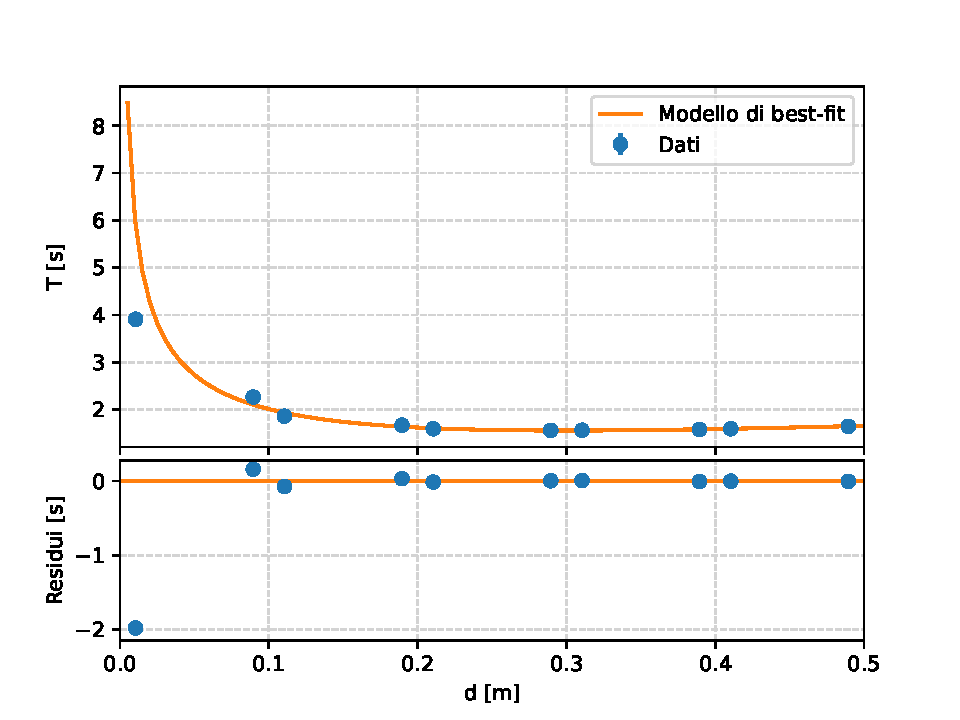
\includegraphics[scale=0.80]{Fit_e_residui.pdf}
	\caption{Grafico di \emph{best}-fit e residui: le incertezze sono presenti ma si vedono poco}
\end{figure}
Siccome in $d=0$ abbiamo un asintoto, gli errori sulle $d$ non sono trascurabili, dunque ho utilizzato il metodo degli errori efficaci (da completare)
Il $\chi^2$ risulta essere pari a 1504: questo potrebbe indicare che all'interno delle nostre misurazioni hanno agito delle fonti di errori sistematici che potrebbero essere dovuti alle forze di attrito o altri fattori. \\
La libreria \texttt{curve\_fit} ha stimato che il parametro libero è circa $\hat{l} = (1.04 \pm 0.01) \, \si{\meter}$ che è un valore compatibile entro le barre di errore con il valore atteso teorico, sebbene un $\chi^2$ così alto potrebbe far ipotizzare che agiscono degli errori sistematici oppure che gli 
\end{document}